\documentclass{standalone}
\usepackage[subpreambles = true]{standalone}

\usepackage{tikz}
\usepackage{circuitikz}
\usetikzlibrary{patterns,decorations.pathmorphing,positioning}

\usepackage{xfrac}  

\begin{document}

	\begin{figure*}[!htp]
		\centering
		\begin{circuitikz} 
%longpot/.style = {pR, resistors/scale=0.75,
%3 resistors/width=1.6, resistors/zigs=6}]

 
\draw (0, 0) node[left=1ex, name=dc_in] {$V_i$} %VI      
to[short, o-] (1, 0);
                         
\draw (1,0)
to[inductor, l={$L_1$}] (4,0)
to[inductor, l=$L_2$] (7,0);

\draw (8.5, 0) node[left=1ex, name=dc_in] [xshift=1cm]{$V_o$} %VI      
to[short, o-] (7, 0);

\draw (4,0) to[capacitor, l=$C$] (4,-3);
\draw (7,0) to[R, l=$R$] (7,-3);
\draw (0,-3) to (8.5,-3);

%\draw (0,0)  to[inductor, l=$L_1$] (4,0)
%to[inductor, l=$L_2$] (12,0);
%
%\draw (4,0)  to[capacitor, l=$C$] (4,-4);
%\draw (10,0)  to[R, l=$R$] (10,-4);


 ;
\end{circuitikz}
		\caption{Sơ đồ bài 2}
		\label{b2-diagram}
	\end{figure*}
	
	\section{Yêu cầu}%-----------------------------
	\begin{itemize}
		\item Xác định mô hình bài toán
		\item Mô phỏng bằng simulink
	\end{itemize}	
	
	
	
	\section{Tính toán giá trị đề cho}%------------------------
	\begin{table}[!htp]
		\centering
		\begin{tabular}{|l|l|l|l|}
			\hline $L_1$ = [1+5] & $L_2$ = [2+3] & C = [6] & R = [7+5]\\
			\hline
		\end{tabular}
		\caption{Bảng các thông số dựa trên MSSV bài 2}
		\label{b2-para-table}
	\end{table}
	%\pagebreak
	
	Dựa vào bảng trên với MSSV là B1907058, ta dễ dàng tính được các thông số cần thiết như bảng sau:\\
	
	\begin{table}[!htp]
		\centering
		\begin{tabular}{|l|l|l|l|}
			\hline $L_1$ = 8mH & $L_2$ = 5mH & C = 9$\upmu$F & R = 6$\Omega$\\
			\hline
		\end{tabular}
		\caption{Bảng các thông số cần thiết bài 2}
		\label{b2-value-table}
	\end{table}
	
	\section{Tính mô hình bài toán}%---------------------------
	Áp dụng định luật Kirchhoff về dòng điện:
	\begin{itemize}
		\item [] $
		\begin{cases}
			i_{L1} - i_{L2} - i_C = 0\\
			i_{L_2} - i_R = 0
		\end{cases}
		$
	\end{itemize}
	
	Biểu diễn dạng chuẩn của mô hình toán:

	\begin{itemize}
		\item [] $	
		\begin{dcases}
			\ddot V_1 &= \dfrac{1}{L_1\,C}\,V_i + \dfrac{1}{L_2\,C}\,V_0 - \left(\dfrac{1}{L_1\,C} + \dfrac{1}{L_2\,C}\right)\,V_1\\
			\dot V_0 &= \dfrac{\dfrac{1}{L_2}\,V_1 - \dfrac{1}{L_2}\,V_0}{R}
		\end{dcases}
		$
	\end{itemize}

	
	\section{Mô phỏng simulink}%---------------------------
	\begin{figure*}[!htp]
		\centering
		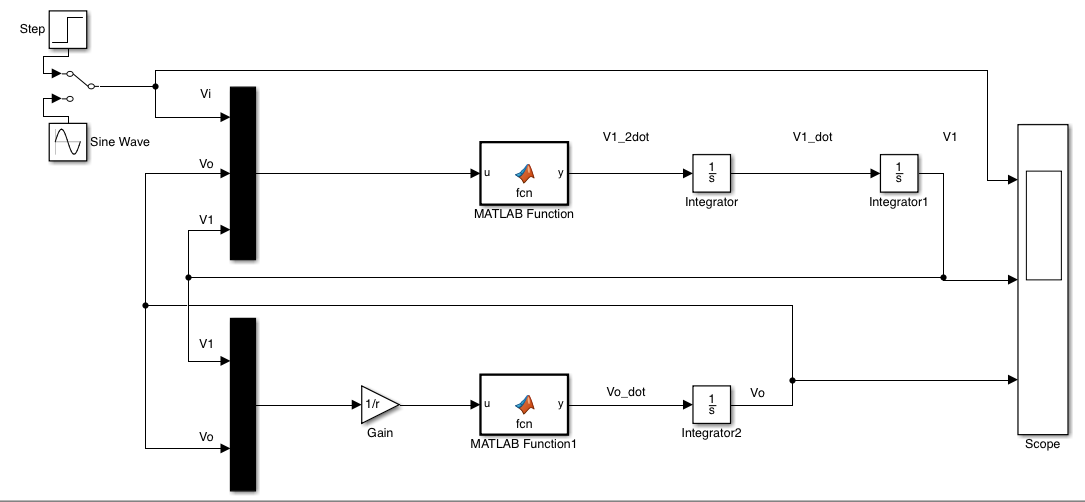
\includegraphics[scale=0.4]{images/b2-simu}
		\caption{Sơ đồ simulink bài 2}
		\label{b2-simu}
	\end{figure*}
	\pagebreak
	
	Với $V_i$ = $sin(\omega t)$.\\
	Giả sử các điều kiện đầu bằng 0. Các thông số được thấy từ bảng \ref{b2-value-table} ở trang \pageref{b2-value-table}.\\

	\begin{figure*}[!htp]
		\centering
		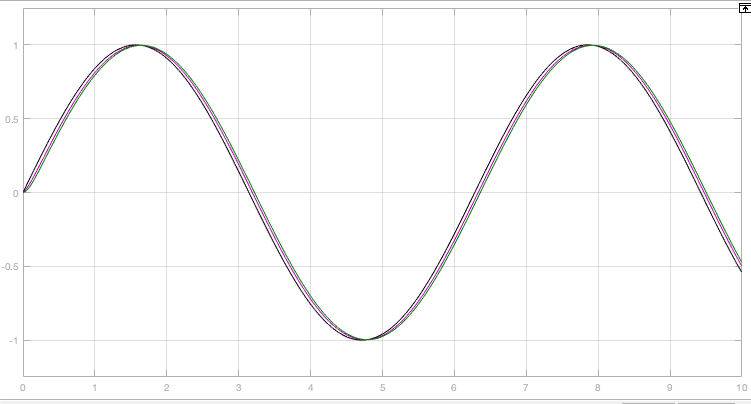
\includegraphics[scale=0.5]{images/b2-scop-sine}
		\caption{Kết quả mô phỏng trên Oscilloscope bài 2 với $V_i$ = $sin(\omega t)$ }
		\label{b2-scop-sine}
	\end{figure*}
	
	Với $V_i$ = u(t) trong đó u(t) là hàm step đơn vị.\\
	Giả sử các điều kiện đầu bằng 0. Các thông số được thấy từ bảng \ref{b2-value-table} ở trang \pageref{b2-value-table}.\\
	%\pagebreak
	\begin{figure*}[!htp]
		\centering
		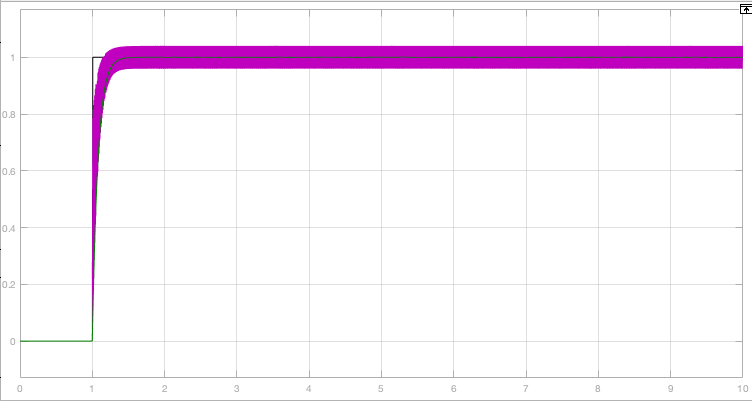
\includegraphics[scale=0.5]{images/b2-scop-step}
		\caption{Kết quả mô phỏng trên Oscilloscope bài 2 với $V_i$ = u(t) }
		\label{b2-scop-step}
	\end{figure*}
	
	
	
	
	
\end{document}